\section{Aufbau des realen Clusters}\label{sec:aufbauCluster}

\citeauthor{zhang2016} haben im Rahmen ihrer gesamten Forschungsarbeit die Plattform Hadoop-Benchmark entwickelt und gemeinsam mit der Selfbalancing-Komponente für Hadoop auf Github zur Verfügung gestellt\footnote{\url{https://github.com/Spirals-Team/hadoop-benchmark}}. Hadoop-Benchmark basiert auf der Software \emph{Docker}\footnote{\url{https://www.docker.com/}} und dem dazugehörigen Tool \emph{Docker Machine}, um damit einfach und schnell ein Hadoop-Cluster aufbauen zu können. Mit \emph{Graphite}\footnote{\url{https://graphiteapp.org/}} ist zudem ein Monitoring-Tool enthalten, mit dem die Performance des Clusters überwacht und analysiert werden kann.

\begin{figure}
    \centering
    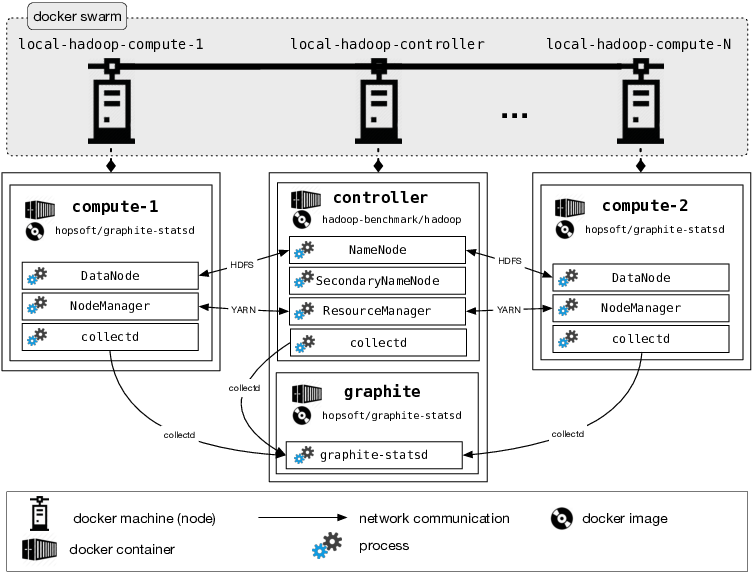
\includegraphics[width=.8\columnwidth]{./images/hadoopBenchmarkArch.png}
    \caption[High-Level-Architektur von Hadoop-Benchmark]{High-Level-Architektur von Hadoop-Benchmark \cite{abb:hadoopBenchmarkArch}}
    \label{fig:hadoopBenchmarkArchitecture}
\end{figure}

Mithilfe von Docker Machine können spezielle Virtuelle Maschinen erstellt werden, die direkt für den Einsatz mit Docker ausgestattet sind. Auf jeder dieser VMs können dadurch direkt ein oder mehrere Docker-Container gestartet werden, welche letztlich das Hadoop-Cluster bilden. Jeder Container enthält neben dem Controller bzw. Node von Hadoop noch das Tool \emph{collectd}\footnote{\url{https://collectd.org/}}, welches das Monitoring des Hadoop-Nodes auf Systemebene übernimmt und die Daten an den Graphite-Container auf der Controller-Machine übermittelt. Es ist dabei möglich, eine beliebige Anzahl an Nodes zu nutzen. Auch ist es möglich, den VMs einen beliebig großen Arbeitsspeicher zur Verfügung zu stellen.

Die Plattform Hadoop-Benchmark enthält auch die bereits in \autoref{sec:lastprofilerstellung} erwähnten Benchmarks Mapreduce Examples, HiBench und SWIM. Sie werden ebenfalls als jeweils eigene Docker-Container gestartet und so an das Cluster übermittelt.

% Wie ist Cluster aufgebaut
% Hilfsscript zur einfachen Verwaltung!